\documentclass[conference]{IEEEtran}
\IEEEoverridecommandlockouts
\usepackage{cite}
\usepackage{amsmath,amssymb,amsfonts,amsthm}
\usepackage{graphicx}
\usepackage{booktabs}
\usepackage{array}
\usepackage{multirow}
\usepackage{xcolor}
\usepackage{pgfplots}
\usetikzlibrary{positioning,shapes.geometric,arrows.meta,fit,backgrounds,calc}
\pgfplotsset{compat=1.17}
\usepackage{microtype}
\usepackage[hidelinks]{hyperref}

\newtheorem{proposition}{Proposition}
\newtheorem{corollary}{Corollary}
\newcommand{\EO}{\mathrm{EO}}
\newcommand{\TPR}{\mathrm{TPR}}
\newcommand{\FPR}{\mathrm{FPR}}

\begin{document}

\title{Beyond Demographic-Free Auditing: Measuring and Mitigating Hidden-Group Bias with Few Labels}


\author{\IEEEauthorblockN{Chirag Joshi, Soumya Shradha, Tanishk Gangwar, Vivansh Garg and Yagya Salwan}
\IEEEauthorblockA{\textit{Department of Computer Science and Engineering}\\
\textit{Manipal University Jaipur}, Jaipur, India\\
}
}

\maketitle

\begin{abstract}
Fairness audits and interventions usually require a protected attribute that practitioners often cannot collect for technical or legal reasons. We study what can be done when demographic data are unavailable except for a small labelled sample. On 8 benchmark dataset-attribute pairs and 10 American Community Survey (ACS) targets, under a pre-registered protocol that never tunes on demographic labels and scores every model at a fixed selection rate, we separate three tasks: finding, measuring and fixing a hidden-group disparity. We first show that, within a true label, a group's mean score gap equals the score's standard deviation times its correlation with the group, divided by the square root of the group's balance. This identity explains why a model trained without the protected attribute shows larger gaps on its own input features than on the hidden group: in 660 demographic-free audits, the protected group never ranked first. Second, about 100 labelled rows suffice to measure the hidden equalized-odds gap; a proxy-weighted estimator is nearly unbiased and 2 to 4 times more accurate than the labelled rows alone, on all 18 targets. Third, mitigation is conditional. On the benchmarks, a 100-label proxy removed 14.5\% of the gap, against at most 7.3\% for demographic-free methods, but on ACS the unguarded proxy did not reliably help, and its benefit tracked the size of the baseline gap. A simple guard that corrects only when the estimated gap is at least 0.08 cut harmful corrections from 26\% to 7\% on ACS and from 29\% to 11\% in a pre-registered replication on five new states.
\end{abstract}

\begin{IEEEkeywords}
algorithmic fairness, fairness without demographics, proxy attributes, fairness auditing, equalized odds, pre-registration
\end{IEEEkeywords}

\section{Introduction}
Most group-fairness methods assume access to a protected attribute $A$, such as race or sex, for every training example \cite{hardt2016equality,agarwal2018reductions,kamiran2012data}. In practice this information is often missing: collecting it is expensive or legally restricted, people may decline to disclose it, or it was never recorded.

Two broad strategies address this problem. \emph{Demographic-free} methods try to improve fairness without any demographic labels, either by giving more weight to examples that are hard to fit \cite{hashimoto2018fairness,lahoti2020fairness,liu2021just,levy2020large} or by penalising features suspected to be linked to $A$ \cite{zhao2022towards}. \emph{Limited-demographics} methods use a small labelled sample to train a proxy for $A$ and then use the proxy to audit the model or to mitigate bias \cite{kenfack2024fairness,awasthi2021evaluating}.

We ask a practical question: \emph{with few or no demographic labels, what can be measured, and when can a disparity be fixed safely?} We separate three tasks that are often treated as one: finding the disadvantaged group, measuring how large the disadvantage is, and reducing it. A method that succeeds at one task need not succeed at the others.

Our evaluation is deliberately conservative. Demographic labels are never used to tune hyper-parameters, and every model is scored at the same selection rate, so no model can look fair simply by predicting the favourable outcome for everyone. The confirmatory experiments follow a pre-registration written after pilots on separate seeds \cite{nosek2018preregistration}.

Our contributions are:
\begin{itemize}
\item \textbf{Why demographic-free audits miss the protected group.} An exact identity links a group's mean score gap to its correlation with the score (Proposition~\ref{prop:identity}). A model trained without $A$ is associated with $A$ only through proxies, so the features it uses most dominate a gap-ranking audit; $A$ ranked first in 0 of 660 audits.
\item \textbf{Measurement from about 100 labels.} A proxy-weighted estimator recovers the hidden equalized-odds gap almost without bias and beat the labelled-rows estimate on all 18 targets, including a pre-registered replication.
\item \textbf{A conditional answer for mitigation.} Proxy correction helped on the benchmarks but needed a guard on ACS: its benefit tracked the baseline gap (Spearman correlation 0.85 over 13 targets), and a simple gap guard held in a held-out test and in a pre-registered replication.
\item \textbf{Negative results.} Selective labelling, tuning on the labelled rows and four demographic-free methods did not give reliable gains.
\end{itemize}

\section{Related Work}
\textbf{Group fairness and mitigation with observed attributes.} Equalized odds and equal opportunity require similar error rates across groups conditional on the true label \cite{hardt2016equality}; we use equalized odds throughout. Mitigation methods are commonly grouped into pre-processing, such as reweighing and massaging of the training data \cite{kamiran2012data}; in-processing, such as the reductions approach that turns a fairness constraint into a sequence of cost-sensitive problems \cite{agarwal2018reductions}; and post-processing of scores or thresholds \cite{hardt2016equality}. All of these assume that $A$ is observed for every training example, which is the assumption this paper relaxes. Our learner is a simple in-processing method with a soft equalized-odds penalty, chosen so that every arm differs only in the group signal it receives, and we reuse the Kamiran-Calders weights inside one of our baselines \cite{kamiran2012data}.

\textbf{Fairness without demographics.} Distributionally robust optimization minimises the loss of the worst-off portion of the data without group labels, either over repeated rounds of loss minimisation \cite{hashimoto2018fairness} or with efficient large-scale CVaR objectives \cite{levy2020large}. ARL trains an adversary that assigns higher weight to examples the learner finds hard \cite{lahoti2020fairness}; JTT upweights examples misclassified by an initial model \cite{liu2021just}; and clustering approaches construct pseudo-groups from learned representations \cite{sohoni2020no}. FairRF instead penalises correlations between predictions and user-specified related features \cite{zhao2022towards}. These methods share a premise: the people a model serves worst coincide with a protected group. Kenfack et al.\ report that they do not necessarily improve demographic parity or equalized odds for the true attribute \cite{kenfack2024fairness}, and hyperparameter selection is a further difficulty when $A$ is unavailable for validation \cite{veldanda2023hyper}. Our score-correlation identity gives a direct reason why the premise can fail: the worst-off regions are defined by the features the model relies on, not by a hidden attribute. We reimplement ARL, CVaR-DRO, JTT and cluster reweighting under one learner so that their comparison with proxy methods is not confounded by architecture or tuning.

\textbf{Limited demographics and proxies.} A second line of work assumes that $A$ is known for a subset of individuals. Kenfack et al.\ train an uncertainty-aware attribute classifier from a labelled subset representing 3\% to 20\% of the data and apply fairness constraints only to rows whose predicted attribute is confident \cite{kenfack2024fairness}. Awasthi et al.\ study fairness evaluation when the attribute predictor is noisy or incomplete, and show that the error of the predictor can bias the estimated disparity in either direction \cite{awasthi2021evaluating}. We work with much smaller labelling budgets, from 25 to 400 rows, keep demographic information out of model tuning, and identify the baseline gap rather than proxy accuracy as the quantity that predicts when proxy-based correction makes a model less fair.

\textbf{Measurement of disparity with an unobserved attribute.} Chen et al.\ analyse proxy-weighted disparity estimators under unawareness and characterise when they over- or under-state the true disparity \cite{chen2019fairness}. Kallus et al.\ derive partial-identification bounds on disparity by combining the main dataset with an auxiliary dataset that contains the protected attribute \cite{kallus2022assessing}. Elzayn et al.\ estimate and enforce conventional fairness metrics using probabilistic protected features \cite{elzayn2023estimating}. Our measurement results sit within this line of work while focusing on very small label budgets, comparing directly against the naive labelled-rows estimate that a practitioner would compute first, and evaluating on two data families.

\textbf{Benchmarks and evaluation practice.} We use standard tabular fairness datasets collected by Le Quy et al.\ \cite{lequy2022survey}. Because older benchmarks such as Adult have been criticised for their age and construction, we also use the ACS Folktables tasks \cite{ding2021retiring}, and we test our main decision rule on ACS states that were not used to design it. Following practice from the experimental sciences, our confirmatory analyses were pre-registered before they were run, with deviations logged \cite{nosek2018preregistration}.

\textbf{Positioning.} Prior work has typically studied either demographic-free or limited-demographics methods, and either measurement or mitigation. We evaluate both families under one learner, one tuning rule and one fixed selection rate; separate the tasks of finding, measuring and fixing a disparity; and connect the outcome of each task to a single quantity, namely how strongly the model's score is associated with the group.

\section{Setup and Methods}
\begin{figure*}[t]
\centering
\resizebox{\textwidth}{!}{%
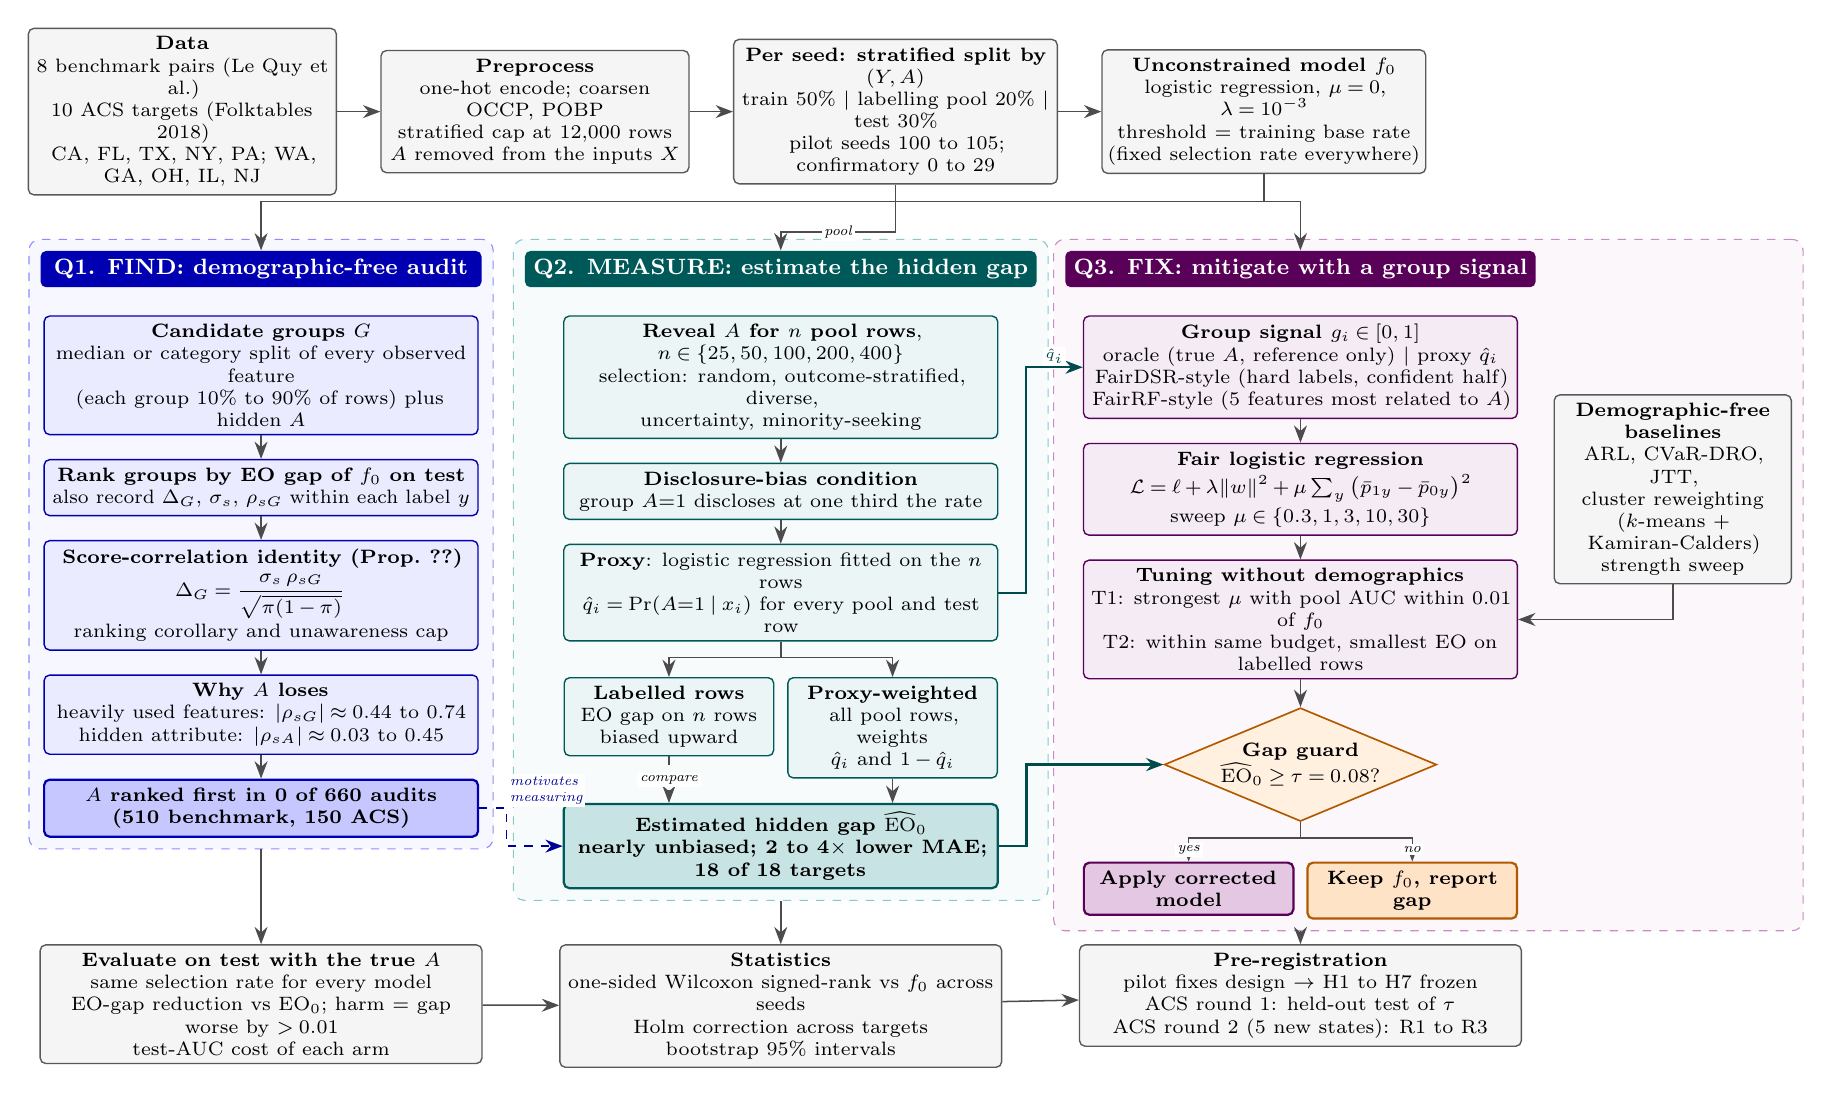
\begin{tikzpicture}[
  font=\scriptsize,
  every node/.append style={execute at begin node={\thinmuskip=3mu\medmuskip=3mu\thickmuskip=4mu}},
  >={Stealth[length=2.2mm]},
  box/.style={draw=#1!70!black, fill=#1!8, rounded corners=2pt, align=flush center, inner sep=3pt, line width=0.5pt},
  box/.default=gray,
  res/.style={draw=#1!70!black, fill=#1!22, rounded corners=2pt, align=flush center, inner sep=3pt, line width=0.8pt, font=\scriptsize\bfseries},
  dec/.style={diamond, aspect=2.4, draw=orange!70!black, fill=orange!12, align=center, inner sep=0.5pt, line width=0.6pt},
  lane/.style={draw=#1!45, fill=#1!3, rounded corners=4pt, line width=0.4pt, dashed},
  head/.style={fill=#1!70!black, text=white, rounded corners=2pt, font=\footnotesize\bfseries, inner sep=3pt, minimum width=5.6cm},
  arr/.style={->, line width=0.55pt, draw=black!70},
  lbl/.style={font=\tiny\itshape, fill=white, inner sep=1pt},
]

% ------------------------------------------------------------ input stage
\node[box=gray, text width=3.7cm] (data) at (0,0)
  {\textbf{Data}\\ 8 benchmark pairs (Le Quy et al.)\\ 10 ACS targets (Folktables 2018)\\ CA, FL, TX, NY, PA; WA, GA, OH, IL, NJ};
\node[box=gray, text width=3.7cm, right=0.55cm of data] (prep)
  {\textbf{Preprocess}\\ one-hot encode; coarsen OCCP, POBP\\ stratified cap at 12{,}000 rows\\ $A$ removed from the inputs $X$};
\node[box=gray, text width=3.9cm, right=0.55cm of prep] (split)
  {\textbf{Per seed: stratified split by $(Y,A)$}\\ train 50\% $\mid$ labelling pool 20\% $\mid$ test 30\%\\ pilot seeds 100 to 105; confirmatory 0 to 29};
\node[box=gray, text width=3.9cm, right=0.55cm of split] (erm)
  {\textbf{Unconstrained model $f_0$}\\ logistic regression, $\mu=0$, $\lambda=10^{-3}$\\ threshold = training base rate\\ (fixed selection rate everywhere)};
\draw[arr] (data) -- (prep);
\draw[arr] (prep) -- (split);
\draw[arr] (split) -- (erm);

% ------------------------------------------------------------ lane headers
\coordinate (L1) at (1.0,-2.0);
\coordinate (L2) at (7.6,-2.0);
\coordinate (L3) at (14.2,-2.0);
\node[head=blue]   (h1) at (L1) {Q1. FIND: demographic-free audit};
\node[head=teal]   (h2) at (L2) {Q2. MEASURE: estimate the hidden gap};
\node[head=violet] (h3) at (L3) {Q3. FIX: mitigate with a group signal};

% ------------------------------------------------------------ lane 1: find
\node[box=blue, text width=5.3cm, below=0.35cm of h1] (f1)
  {\textbf{Candidate groups $G$}\\ median or category split of every observed feature\\ (each group 10\% to 90\% of rows) plus hidden $A$};
\node[box=blue, text width=5.3cm, below=0.3cm of f1] (f2)
  {\textbf{Rank groups by EO gap of $f_0$ on test}\\ also record $\Delta_G$, $\sigma_s$, $\rho_{sG}$ within each label $y$};
\node[box=blue, text width=5.3cm, below=0.3cm of f2] (f3)
  {\textbf{Score-correlation identity (Prop.~\ref{prop:identity})}\\[1pt]
   $\displaystyle \Delta_G=\frac{\sigma_s\,\rho_{sG}}{\sqrt{\pi(1-\pi)}}$\\[1pt]
   ranking corollary and unawareness cap};
\node[box=blue, text width=5.3cm, below=0.3cm of f3] (f4)
  {\textbf{Why $A$ loses}\\ heavily used features: $|\rho_{sG}|\approx0.44$ to $0.74$\\ hidden attribute: $|\rho_{sA}|\approx0.03$ to $0.45$};
\node[res=blue, text width=5.3cm, below=0.3cm of f4] (f5)
  {$A$ ranked first in 0 of 660 audits\\ (510 benchmark, 150 ACS)};
\draw[arr] (f1) -- (f2);
\draw[arr] (f2) -- (f3);
\draw[arr] (f3) -- (f4);
\draw[arr] (f4) -- (f5);

% ------------------------------------------------------------ lane 2: measure
\node[box=teal, text width=5.3cm, below=0.35cm of h2] (m1)
  {\textbf{Reveal $A$ for $n$ pool rows}, $n\in\{25,50,100,200,400\}$\\ selection: random, outcome-stratified, diverse,\\ uncertainty, minority-seeking};
\node[box=teal, text width=5.3cm, below=0.3cm of m1] (m1b)
  {\textbf{Disclosure-bias condition}\\ group $A{=}1$ discloses at one third the rate};
\node[box=teal, text width=5.3cm, below=0.3cm of m1b] (m2)
  {\textbf{Proxy}: logistic regression fitted on the $n$ rows\\ $\hat q_i=\Pr(A{=}1\mid x_i)$ for every pool and test row};
\node[box=teal, text width=2.45cm, below=0.45cm of m2, xshift=-1.42cm] (m3a)
  {\textbf{Labelled rows}\\ EO gap on $n$ rows\\ biased upward};
\node[box=teal, text width=2.45cm, below=0.45cm of m2, xshift=1.42cm] (m3b)
  {\textbf{Proxy-weighted}\\ all pool rows, weights\\ $\hat q_i$ and $1-\hat q_i$};
\node[res=teal, text width=5.3cm, below=2.05cm of m2] (m4)
  {Estimated hidden gap $\widehat{\EO}_0$\\ nearly unbiased; 2 to 4$\times$ lower MAE; 18 of 18 targets};
\draw[arr] (m1) -- (m1b);
\draw[arr] (m1b) -- (m2);
\draw[arr] (m2.south) -- ++(0,-0.2) -| (m3a.north);
\draw[arr] (m2.south) -- ++(0,-0.2) -| (m3b.north);
\draw[arr, dashed] (m3a.south) -- (m3a.south |- m4.north) node[midway, lbl] {compare};
\draw[arr] (m3b.south) -- (m3b.south |- m4.north);

% ------------------------------------------------------------ lane 3: fix
\node[box=violet, text width=5.3cm, below=0.35cm of h3] (x1)
  {\textbf{Group signal $g_i\in[0,1]$}\\ oracle (true $A$, reference only) $\mid$ proxy $\hat q_i$\\ FairDSR-style (hard labels, confident half)\\ FairRF-style (5 features most related to $A$)};
\node[box=violet, text width=5.3cm, below=0.3cm of x1] (x2)
  {\textbf{Fair logistic regression}\\[1pt]
   $\mathcal{L}=\ell+\lambda\|w\|^2+\mu\sum_{y}\big(\bar p_{1y}-\bar p_{0y}\big)^2$\\[1pt]
   sweep $\mu\in\{0.3,1,3,10,30\}$};
\node[box=violet, text width=5.3cm, below=0.3cm of x2] (x3)
  {\textbf{Tuning without demographics}\\ T1: strongest $\mu$ with pool AUC within 0.01 of $f_0$\\ T2: within same budget, smallest EO on labelled rows};
\node[dec, below=0.35cm of x3] (x4)
  {\textbf{Gap guard}\\ $\widehat{\EO}_0\ge\tau=0.08$?};
\node[res=violet, text width=2.45cm, below=0.5cm of x4, xshift=-1.42cm] (x5a) {Apply corrected model};
\node[res=orange, text width=2.45cm, below=0.5cm of x4, xshift=1.42cm] (x5b) {Keep $f_0$, report gap};
\draw[arr] (x1) -- (x2);
\draw[arr] (x2) -- (x3);
\draw[arr] (x3) -- (x4);
\draw[arr] (x4.south) -- ++(0,-0.2) -| (x5a.north) node[pos=0.75, lbl] {yes};
\draw[arr] (x4.south) -- ++(0,-0.2) -| (x5b.north) node[pos=0.75, lbl] {no};

% demographic-free baselines, side box feeding the same tuning step
\node[box=gray, text width=2.8cm, right=0.45cm of x2] (dfb)
  {\textbf{Demographic-free baselines}\\ ARL, CVaR-DRO, JTT,\\ cluster reweighting\\ ($k$-means + Kamiran-Calders)\\ strength sweep};
\draw[arr] (dfb.south) |- (x3.east);

% ------------------------------------------------------------ lane backgrounds
\begin{scope}[on background layer]
  \node[lane=blue,   fit=(h1)(f1)(f5), inner sep=4pt] (bg1) {};
  \node[lane=teal,   fit=(h2)(m1)(m4), inner sep=4pt] (bg2) {};
  \node[lane=violet, fit=(h3)(x1)(x5a)(x5b)(dfb), inner sep=4pt] (bg3) {};
\end{scope}

% ------------------------------------------------------------ links from the input stage
\draw[arr] (erm.south) -- ++(0,-0.35) -| (h1.north);
\draw[arr] (erm.south) -- ++(0,-0.35) -| (h3.north);
\draw[arr] (split.south) -- ++(0,-0.6) -| (h2.north) node[pos=0.25, lbl] {pool};

% cross-lane links
\draw[arr, teal!60!black, line width=0.8pt] (m2.east) -- ++(0.35,0) |- (x1.west) node[pos=0.75, lbl, above] {$\hat q_i$};
\draw[arr, teal!60!black, line width=0.8pt] (m4.east) -- ++(0.35,0) |- (x4.west -| bg3.west) -- (x4.west);
\draw[arr, blue!60!black, dashed] (f5.east) -- ++(0.35,0) node[lbl, above, pos=1.0, anchor=south west, align=left] {motivates\\ measuring}  |- (m4.west);

% ------------------------------------------------------------ evaluation stage
\coordinate (bot) at ($(bg2.south)+(0,-0.55)$);
\node[box=gray, text width=5.4cm, anchor=north] (ev) at ($(bot -| L1)$)
  {\textbf{Evaluate on test with the true $A$}\\ same selection rate for every model\\ EO-gap reduction vs $\EO_0$; harm = gap worse by $>0.01$\\ test-AUC cost of each arm};
\node[box=gray, text width=5.4cm, anchor=north] (st) at ($(bot -| L2)$)
  {\textbf{Statistics}\\ one-sided Wilcoxon signed-rank vs $f_0$ across seeds\\ Holm correction across targets\\ bootstrap 95\% intervals};
\node[box=gray, text width=5.4cm, anchor=north] (pr) at ($(bot -| L3)$)
  {\textbf{Pre-registration}\\ pilot fixes design $\rightarrow$ H1 to H7 frozen\\ ACS round 1: held-out test of $\tau$\\ ACS round 2 (5 new states): R1 to R3};
\draw[arr] (ev) -- (st);
\draw[arr] (st) -- (pr);
\draw[arr] (bg1.south) -- (ev.north);
\draw[arr] (bg2.south) -- (st.north);
\draw[arr] (bg3.south -| pr.north) -- (pr.north);

\end{tikzpicture}%
}
\caption{End-to-end study design. The hidden attribute $A$ is removed from every model input and used only for the labelled sample and for final grading. Each seed feeds three questions: Q1 asks whether a demographic-free audit can \emph{find} the disadvantaged group (Section~\ref{sec:audit}); Q2 asks whether $n$ revealed labels and a proxy can \emph{measure} the hidden equalized-odds gap; Q3 asks whether the same signal can \emph{fix} it, comparing proxy, oracle, FairDSR- and FairRF-style variants and four demographic-free baselines under one learner and one tuning rule. The measured gap from Q2 gates the correction in Q3 through the gap guard. All arms are graded on the test split with the true $A$ at a fixed selection rate.}
\label{fig:pipeline}
\end{figure*}

Fig.~\ref{fig:pipeline} gives an overview of the full study design.

\subsection{Notation and metric}
Each example has features $X$, a binary label $Y$ and a binary protected attribute $A$ that is \emph{never} used as a model input. A classifier produces a score $s$ and a decision $\hat Y$, with the threshold chosen so that the selection rate matches the training base rate. Writing $\TPR_a$ and $\FPR_a$ for the true- and false-positive rates in group $A=a$, the equalized-odds gap is
\begin{equation}
\EO=\max\big(\,|\TPR_1-\TPR_0|,\;|\FPR_1-\FPR_0|\,\big).
\end{equation}
We report the relative reduction against the unconstrained model's gap $\EO_0$, and absolute changes when $\EO_0$ is small.

\subsection{Learner and group signals}
All mitigation arms use the same learner, logistic regression with predicted probabilities $p_i$ and the loss
\begin{equation}
\mathcal{L}=\frac{1}{n}\sum_{i}\ell(p_i,y_i)+\lambda\|w\|^2+\mu\sum_{y\in\{0,1\}}\big(\bar p_{1y}-\bar p_{0y}\big)^2,
\end{equation}
where $\bar p_{ay}$ is the mean of $p_i$ over examples with label $y$ in group $a$, weighted by a group signal $g_i\in[0,1]$ (and by $1-g_i$ for $a=0$).

The arms differ only in how $g$ is obtained. The \emph{oracle} uses the true attribute and serves only as a reference. The \emph{proxy} uses $\hat q_i$, the probability of $A=1$ predicted by a logistic regression fitted on $n$ labelled rows. We also test a FairDSR-style variant that uses hard proxy labels on the more confident half of rows \cite{kenfack2024fairness}, and a FairRF-style variant that penalises the five features most correlated with $A$ in the labelled rows \cite{zhao2022towards}.

\subsection{Demographic-free baselines}
ARL with a linear learner and adversary \cite{lahoti2020fairness}, CVaR-DRO \cite{levy2020large}, JTT \cite{liu2021just}, and cluster reweighting each receive a sweep over their strength parameter. Cluster reweighting uses $k$-means pseudo-groups with Kamiran-Calders weights \cite{kamiran2012data}.

\subsection{Choosing which rows to label}
Demographics are revealed only for rows selected from a labelling pool. The pilot compared random, outcome-stratified, diverse ($k$-means centres), uncertainty-based and minority-seeking selection; the confirmatory runs keep random and outcome-stratified selection. We also consider a disclosure-bias condition in which members of the protected group disclose at one third the rate of others.

\subsection{Tuning without demographics}
For each arm, we keep the strongest setting whose pool AUC stays within 0.01 of the unconstrained model (rule T1). If no setting satisfies this constraint, we keep the unconstrained model. A label-informed rule (T2) instead selects, within the same AUC budget, the setting with the smallest EO gap on the labelled rows.

\subsection{Measuring the hidden gap}
Both estimators use the unconstrained model's decisions on the pool. The \emph{labelled-rows} estimator computes the EO gap using only the $n$ labelled rows. The \emph{proxy-weighted} estimator uses every pool row, weighting it by $\hat q_i$ for group 1 and by $1-\hat q_i$ for group 0; for example,
\begin{equation}
\widehat{\TPR}_1=\frac{\sum_{i:\,y_i=1}\hat q_i\,\hat y_i}{\sum_{i:\,y_i=1}\hat q_i},
\end{equation}
and similarly for the other three rates.

\subsection{Gap guard}
Proxy correction is applied only if the proxy-weighted estimate of $\EO_0$ is at least $\tau$; otherwise, the unconstrained model is kept. The threshold $\tau=0.08$ was chosen on the benchmark data and fixed before any ACS run.

\section{Why Demographic-Free Audits Miss the Protected Group}\label{sec:audit}
A demographic-free audit ranks candidate groups, usually defined by observed features, according to their error or score gap and flags the largest one. The following identity shows what this ranking actually measures. Fix a label $y$, and let $\pi$ be the share of group $G$ among examples with that label.

\begin{proposition}[Score-correlation identity]\label{prop:identity}
For any score $s$ and binary group $G$ with $0<\pi<1$,
\begin{equation}
\Delta_G=\frac{\sigma_s\,\rho_{sG}}{\sqrt{\pi(1-\pi)}},
\end{equation}
where $\Delta_G$ is the difference in mean score between $G=1$ and $G=0$, $\sigma_s$ is the standard deviation of $s$, and $\rho_{sG}$ is the correlation of $s$ with the indicator of $G$, all within label $y$.
\end{proposition}

\begin{proof}
Within label $y$, the covariance of $s$ and $G$ equals $\pi(1-\pi)\Delta_G$, and the standard deviation of $G$ is $\sqrt{\pi(1-\pi)}$. Dividing the covariance by $\sigma_s\sqrt{\pi(1-\pi)}$ gives $\rho_{sG}$.
\end{proof}

\begin{corollary}[Ranking]
The protected group outranks a feature group $G$ only if
\begin{equation}
\frac{|\rho_{sA}|}{\sqrt{\pi_A(1-\pi_A)}}>\frac{|\rho_{sG}|}{\sqrt{\pi_G(1-\pi_G)}}.
\end{equation}
If the score rises with one roughly Gaussian feature, the median split of that feature has $|\rho_{sG}|\approx0.80$, so a group making up 15\% of rows needs $|\rho_{sA}|>0.57$.
\end{corollary}

\begin{corollary}[Unawareness cap]
If the model does not take $A$ as input, $|\rho_{sA}|$ is at most the maximal correlation between $A$ and any function of the features. The protected group can top the audit only when the features nearly reveal it.
\end{corollary}

The practical implication is that the audit is largely measuring how strongly the model's score depends on each candidate group indicator. Features that the model uses heavily therefore tend to produce large gaps. A hidden attribute can rank highly only when the observed features provide a strong proxy for it.

Table~\ref{tab:audit} confirms this pattern on both data families. The identity held to within $1.2\times10^{-14}$ numerically, and on the benchmarks the ranking by mean score gap agreed with the ranking by thresholded EO gap (Spearman 0.85).

\begin{table}[t]
\caption{Demographic-free audit of an unconstrained model: rank of the hidden attribute among feature-defined groups (1 = largest EO gap) and score correlations. Medians or means over 30 seeds.}
\label{tab:audit}
\centering
\footnotesize
\setlength{\tabcolsep}{3pt}
\begin{tabular}{@{}lcccc@{}}
\toprule
Target & EO gap of $A$ & Rank of $A$ & $|\rho_{sA}|$ & max $|\rho_{sG}|$ \\
\midrule
Law $\cdot$ race & 0.39 & 6 of 8 & 0.45 & 0.74 \\
COMPAS $\cdot$ race & 0.25 & 5 of 5 & 0.28 & 0.53 \\
German $\cdot$ age & 0.17 & 16.5 of 37 & 0.14 & 0.54 \\
Credit $\cdot$ age & 0.17 & 12 of 22 & 0.14 & 0.74 \\
Adult $\cdot$ sex & 0.16 & 14 of 18 & 0.24 & 0.67 \\
COMPAS $\cdot$ sex & 0.14 & 5 of 5 & 0.13 & 0.55 \\
OULAD $\cdot$ disability & 0.11 & 16 of 24 & 0.09 & 0.51 \\
Dutch $\cdot$ sex & 0.05 & 15 of 19 & 0.04 & 0.61 \\
\midrule
ACS CA $\cdot$ race & 0.06 & 19 & 0.09 & 0.44 \\
ACS FL $\cdot$ race & 0.11 & 16 & 0.10 & 0.49 \\
ACS TX $\cdot$ race & 0.06 & 18 & 0.07 & 0.49 \\
ACS NY $\cdot$ sex & 0.02 & 22 & 0.03 & 0.44 \\
ACS PA $\cdot$ sex & 0.06 & 17 & 0.07 & 0.70 \\
\midrule
\multicolumn{5}{@{}l}{$A$ ranked first: 0 of 510 benchmark audits (17 pairs); 0 of 150 ACS audits.}\\
\bottomrule
\end{tabular}
\vspace{2pt}

\raggedright\scriptsize ACS audits had 19 to 23 candidate groups, including $A$. Nine further benchmark pairs (Bank, Diabetes and the second attribute of Adult, German, Law, Credit and OULAD) are included in the 510 audits.
\end{table}

\section{Experimental Protocol}
\textbf{Data.} Table~\ref{tab:data} lists the targets. Benchmarks come from the collection of Le Quy et al.\ \cite{lequy2022survey}; ACS data come from Folktables (2018, one-year person survey) \cite{ding2021retiring}, with occupation coarsened to major groups and place of birth to US-born or abroad region. Datasets above 12{,}000 rows were subsampled (stratified) to 12{,}000.

\begin{table}[t]
\caption{Targets. Favourable label in parentheses; $A{=}1$ denotes the group listed.}
\label{tab:data}
\centering
\scriptsize
\setlength{\tabcolsep}{2.5pt}
\begin{tabular}{@{}lllr@{}}
\toprule
Source & Label & Hidden attribute ($A{=}1$) & Rows \\
\midrule
Adult & income $>$50K & sex (female) & 12{,}000 \\
COMPAS & no 2-yr recidivism & race (Afr.-Am.); sex (female) & 5{,}278 \\
Law School & passes bar & race (non-white) & 12{,}000 \\
Credit (Taiwan) & no default & age $<$25 & 12{,}000 \\
OULAD & passes course & disability & 12{,}000 \\
Dutch census & high occupation & sex (female) & 12{,}001 \\
German credit & good credit & age $<$25 & 1{,}000 \\
\midrule
ACS round 1 & income / employment & CA, FL, TX race; NY, PA sex & 12{,}000 \\
ACS round 2 & income / employment & WA, GA, OH race; IL, NJ sex & 12{,}000 \\
\bottomrule
\end{tabular}
\end{table}

\textbf{Splits and seeds.} Each seed splits the data into training (50\%), a labelling pool (20\%) and test (30\%), stratified by label and attribute. Label budgets are $n\in\{25,50,100,200,400\}$, capped at half the pool. Penalty strengths are $\mu\in\{0.3,1,3,10,30\}$ with $\lambda=10^{-3}$.

\textbf{Pre-registration.} A pilot on seeds 100 to 105 compared the five labelling strategies and fixed the design; seven hypotheses (H1 to H7) were then frozen before confirmatory seeds 0 to 29. Two deviations were logged: extra backfire pairs used 10 seeds instead of 30, and some runs were split across processes. ACS round 1 tested the frozen guard threshold out of sample; ACS round 2 (five new states) was pre-registered with three hypotheses (R1 to R3) before it was run. Tests are one-sided Wilcoxon signed-rank tests across seeds against the unconstrained model, Holm-corrected across targets, with bootstrap 95\% intervals.

\section{Results}
\subsection{Measurement: about 100 labels suffice}
Table~\ref{tab:measure} compares the two estimators of the unconstrained model's hidden gap. The labelled-rows estimate is strongly biased upward at small $n$. The reason is that taking the absolute value of a noisy difference turns sampling variation into apparent unfairness. The proxy-weighted estimate is nearly unbiased and 2 to 4 times more accurate at $n\le100$.

The same pattern appears in the pre-registered ACS round 2. At $n=100$, the proxy-weighted estimator was more accurate on all 5 new targets, with mean absolute error ranging from 0.03 to 0.06, compared with 0.08 to 0.16 for the labelled-rows estimate (R1 supported).

\begin{table}[t]
\caption{Estimating the unconstrained model's hidden EO gap from $n$ labelled rows: mean absolute error (MAE) and bias. L = labelled rows only; P = proxy-weighted. 30 seeds.}
\label{tab:measure}
\centering
\footnotesize
\setlength{\tabcolsep}{2.6pt}
\begin{tabular}{@{}r cccc cccc@{}}
\toprule
& \multicolumn{4}{c}{Benchmarks (8 targets)} & \multicolumn{4}{c}{ACS round 1 (5 targets)} \\
\cmidrule(lr){2-5}\cmidrule(l){6-9}
$n$ & MAE L & MAE P & Bias L & Bias P & MAE L & MAE P & Bias L & Bias P \\
\midrule
25 & 0.284 & 0.093 & +0.234 & $-$0.001 & 0.241 & 0.059 & +0.235 & +0.037 \\
50 & 0.226 & 0.097 & +0.174 & $-$0.004 & 0.175 & 0.047 & +0.173 & +0.023 \\
100 & 0.163 & 0.072 & +0.128 & 0.000 & 0.117 & 0.041 & +0.111 & +0.013 \\
200 & 0.107 & 0.061 & +0.065 & $-$0.007 & 0.076 & 0.037 & +0.062 & +0.009 \\
400 & 0.078 & 0.053 & +0.038 & $-$0.002 & 0.053 & 0.030 & +0.034 & $-$0.001 \\
\bottomrule
\end{tabular}
\end{table}

\subsection{Mitigation on the benchmarks}
Fig.~\ref{fig:budget} shows mean EO-gap reduction against the label budget on the 7 benchmark targets that allow every budget. With 100 random labels, the proxy reduced the gap by 15.5\% [12.6, 18.2], compared with 6.9\% for the best demographic-free method, cluster reweighting, and 27.0\% for the oracle. ARL, CVaR-DRO and JTT remained between $-$2.5\% and 1.6\%.

Table~\ref{tab:bench} gives the per-target results. The proxy matched the oracle on Adult and Law, recovered roughly half to four fifths of the oracle improvement on Credit and COMPAS, but struggled with OULAD, where the proxy was weak, and Dutch, where it actually reversed the gap. After Holm correction, the 100-label proxy was significant on 4 of 8 targets, the 400-label proxy on 6 of 7, the oracle on 7 of 8 and cluster reweighting on 3 of 8. Because the AUC budget is enforced on the pool, the realised test-AUC cost averaged at most 1.3 points for any arm and target.

\begin{figure}[t]
\centering
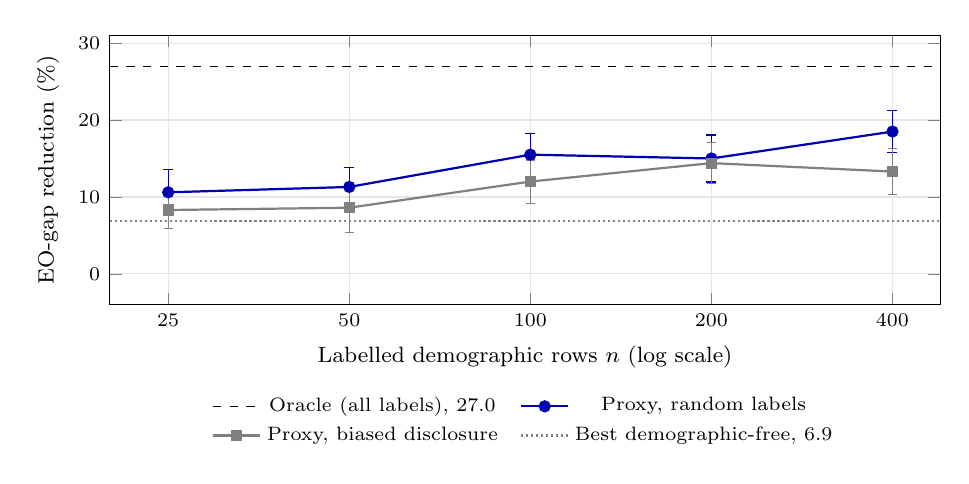
\begin{tikzpicture}
\begin{axis}[
width=\columnwidth, height=5.0cm,
xmode=log, log basis x=2,
xtick={25,50,100,200,400}, xticklabels={25,50,100,200,400},
xmin=20, xmax=480, ymin=-4, ymax=31,
xlabel={Labelled demographic rows $n$ (log scale)},
ylabel={EO-gap reduction (\%)},
ylabel style={font=\footnotesize}, xlabel style={font=\footnotesize},
tick label style={font=\scriptsize},
legend style={font=\scriptsize, at={(0.5,-0.30)}, anchor=north, draw=none, legend columns=2, /tikz/every even column/.append style={column sep=6pt}},
grid=major, grid style={gray!20},
]
\addplot[black, dashed, domain=20:480, samples=2] {27.0};
\addlegendentry{Oracle (all labels), 27.0}
\addplot[blue!70!black, thick, mark=*, mark size=1.8pt, error bars/.cd, y dir=both, y explicit]
coordinates {(25,10.6) +- (0,2.95) (50,11.3) +- (0,2.5) (100,15.5) +- (0,2.8) (200,15.0) +- (0,3.05) (400,18.5) +- (0,2.7)};
\addlegendentry{Proxy, random labels}
\addplot[gray, thick, mark=square*, mark size=1.6pt, error bars/.cd, y dir=both, y explicit]
coordinates {(25,8.3) +- (0,2.4) (50,8.6) +- (0,3.25) (100,12.0) +- (0,2.8) (200,14.4) +- (0,2.65) (400,13.3) +- (0,3.0)};
\addlegendentry{Proxy, biased disclosure}
\addplot[gray, densely dotted, thick, domain=20:480, samples=2] {6.9};
\addlegendentry{Best demographic-free, 6.9}
\end{axis}
\end{tikzpicture}
\caption{Mean EO-gap reduction over 7 benchmark targets (German excluded: its pool cannot supply 200 or more labels), tuned without demographics within a 1-point AUC budget. Error bars: 95\% bootstrap intervals over 30 seeds. ARL 1.3, CVaR-DRO 1.6, JTT $-$2.5.}
\label{fig:budget}
\end{figure}

\begin{table}[t]
\caption{Benchmark EO-gap reduction (\%) at a 1-point AUC budget, 30 seeds. CR = cluster reweighting (best demographic-free method).}
\label{tab:bench}
\centering
\footnotesize
\setlength{\tabcolsep}{3pt}
\begin{tabular}{@{}lccccc@{}}
\toprule
Target & EO$_0$ & CR & Proxy 100 [95\% CI] & Proxy 400 & Oracle \\
\midrule
Law $\cdot$ race & 0.39 & 1 & 30 [25, 35] & 31 & 32 \\
COMPAS $\cdot$ race & 0.25 & 4 & 9 [6, 13] & 11 & 11 \\
German $\cdot$ age & 0.17 & 10 & 8 [$-$4, 16] & n/a & 2 \\
Credit $\cdot$ age & 0.17 & 31 & 20 [11, 27] & 36 & 34 \\
Adult $\cdot$ sex & 0.16 & 28 & 48 [39, 55] & 56 & 51 \\
COMPAS $\cdot$ sex & 0.14 & 3 & 5 [$-$1, 11] & 12 & 11 \\
OULAD $\cdot$ disab. & 0.11 & $-$4 & 2 [$-$4, 8] & 10 & 32 \\
Dutch $\cdot$ sex & 0.05 & $-$16 & $-$5 [$-$17, 7] & $-$26 & 19 \\
\midrule
Mean (8) & & 7.3 & 14.5 & & 23.9 \\
\bottomrule
\end{tabular}
\end{table}

\subsection{ACS: the gap decides, and the guard holds}
On ACS round 1, the unguarded proxy did not reproduce the benchmark result. At $n=100$, it averaged $-$4.1\% reduction compared with 8.1\% for cluster reweighting, while the oracle still removed 31\% to 58\% of the gap on the four targets with $\EO_0\ge0.05$.

The ACS proxies were uniformly weak, with proxy AUC between 0.58 and 0.70 at 100 to 400 labels. Proxy strength alone, however, did not explain the failures. NY $\cdot$ sex had one of the stronger proxies but produced the worst result. The baseline gap was much more informative. Across the 13 benchmark and round-1 targets (12 at 400 labels), $\EO_0$ predicted the absolute benefit of both the 100-label and 400-label proxies, with Spearman correlation 0.85 in each case. When $\EO_0<0.05$, correction made the gap worse in 38\% of runs at 100 labels and 60\% at 400 labels, compared with 15\% and 5\% for larger baseline gaps.

Table~\ref{tab:acs} reports the gap guard on all 10 ACS targets. In round 1, which served as a held-out test of the frozen threshold, the guard reduced the harm rate from 26\% to 7\% at 100 labels and from 18\% to 1\% at 400 labels. Mean reduction consequently increased from $-$4.1\% to 1.6\% at 100 labels and from 1.3\% to 9.7\% at 400 labels. In the pre-registered round 2, harm fell from 29\% to 11\% at 100 labels and from 23\% to 5\% at 400 labels (R2 supported), while the guarded 400-label proxy reduced the gap by 10.8\% on targets with $\EO_0\ge0.05$ (R3 supported).

\begin{table}[t]
\caption{ACS, 400 labels: EO-gap reduction (\%) and harm rate (gap worse by $>0.01$) without (U) and with (G) the 0.08 gap guard. 30 seeds per target.}
\label{tab:acs}
\centering
\footnotesize
\setlength{\tabcolsep}{4pt}
\begin{tabular}{@{}llccccc@{}}
\toprule
& Target & EO$_0$ & Red.\ U & Red.\ G & Harm U & Harm G \\
\midrule
\multirow{5}{*}{\rotatebox{90}{Round 1}} & FL $\cdot$ race & 0.108 & 39.2 & 31.9 & 0.00 & 0.00 \\
& TX $\cdot$ race & 0.057 & 26.1 & 13.0 & 0.07 & 0.00 \\
& CA $\cdot$ race & 0.056 & 36.4 & 11.4 & 0.00 & 0.00 \\
& PA $\cdot$ sex & 0.055 & $-$0.6 & 0.0 & 0.20 & 0.00 \\
& NY $\cdot$ sex & 0.022 & $-$94.4 & $-$8.1 & 0.63 & 0.03 \\
\midrule
\multirow{5}{*}{\rotatebox{90}{Round 2}} & NJ $\cdot$ sex & 0.080 & 0.1 & 0.0 & 0.10 & 0.00 \\
& GA $\cdot$ race & 0.061 & 44.5 & 26.7 & 0.07 & 0.00 \\
& WA $\cdot$ race & 0.058 & 21.9 & 5.6 & 0.13 & 0.03 \\
& OH $\cdot$ race & 0.044 & 5.7 & $-$0.2 & 0.17 & 0.03 \\
& IL $\cdot$ sex & 0.027 & $-$96.4 & $-$28.4 & 0.67 & 0.17 \\
\bottomrule
\end{tabular}
\vspace{2pt}

\raggedright\scriptsize Pooled harm rate, unguarded to guarded: round 1, 0.26 to 0.07 (100 labels) and 0.18 to 0.01 (400 labels); round 2, 0.29 to 0.11 and 0.23 to 0.05.
\end{table}

The guard is not free. It trades some potential improvement for safety: GA falls from 44.5\% to 26.7\%, while CA falls from 36.4\% to 11.4\%. It also does not completely eliminate harm when the baseline gap is close to zero, as seen for IL $\cdot$ sex. Finally, a large gap is not sufficient on its own. NJ $\cdot$ sex starts with $\EO_0=0.08$ but shows essentially no improvement.

\subsection{Pre-registered outcomes and negative results}
Table~\ref{tab:hyp} summarizes the confirmatory hypotheses. Four of seven benchmark hypotheses and all three round-2 hypotheses were supported.

Several negative findings matter as much. First, choosing which rows to label did not provide a clear advantage. In the pilot, uncertainty, minority-seeking, and diverse selection averaged 9.7\% to 11.4\% reduction, compared with 13.8\% for random selection. Second, tuning on the labelled rows (T2) was 3.7 to 5.3 points worse than demographic-free tuning on the benchmarks, but 2.7 to 6.8 points better on ACS. Neither rule therefore dominated across datasets. Third, a pre-registered backfire diagnostic comparing the direction of the true-group and proxy-group gaps predicted harm only weakly (AUROC 0.58). This result motivated the simpler gap guard.

Disclosure bias consistently reduced the benefit, by 3.0 to 5.1 points on the benchmarks and 7.4 to 13.7 points on ACS. A neural-network check was inconclusive because even the oracle failed to improve under the chosen penalty grid.

\begin{table}[t]
\caption{Confirmatory hypotheses and outcomes.}
\label{tab:hyp}
\centering
\footnotesize
\setlength{\tabcolsep}{3pt}
\begin{tabular}{@{}>{\raggedright\arraybackslash}p{5.45cm}>{\raggedright\arraybackslash}p{2.8cm}@{}}
\toprule
Hypothesis & Outcome \\
\midrule
H1: 100-label proxy beats every demographic-free method (benchmarks) & Supported (14.5 vs $\le$7.3) \\
H2: 400-label proxy reaches 75\% of oracle & Not supported (68\%) \\
H3: stratified selection within 3 points of random & Supported \\
H4: disclosure bias lowers the benefit & Supported \\
H5: T2 not better than T1 at $n\le100$ & Supported \\
H6: direction diagnostic predicts harm (AUROC $>$0.70) & Not supported (0.58) \\
H7: neural proxy beats ARL and JTT & Inconclusive \\
\midrule
R1: proxy-weighted estimate better on $\ge$4 of 5 new targets & Supported (5 of 5) \\
R2: gap guard lowers harm at 100 and 400 labels & Supported \\
R3: guarded proxy positive where $\EO_0\ge0.05$ & Supported (10.8\%) \\
\bottomrule
\end{tabular}
\end{table}

\section{Discussion and Limitations}
\textbf{Implications.} For auditors, a modest demographic survey of about 100 people combined with a population-wide proxy is enough to estimate equalized-odds gaps within a few points. Searching for the disadvantaged group without demographic labels, by contrast, tends to find the model's own features rather than the hidden protected group.

For practitioners, the key takeaway is to measure the gap before trying to correct it. When the baseline disparity is large, proxy correction can bring a meaningful improvement. When the estimated gap is small, correction with a weak proxy mostly adds noise and can even reverse the disparity, so the measured gap is a useful gate for deciding whether to intervene.

\textbf{Limitations.} The protected attributes in our experiments are binary, so intersectional and multi-group settings remain untested. The proxies and primary learner are linear, and our neural-network check was inconclusive. ARL, CVaR-DRO, JTT and the FairDSR- and FairRF-style variants are our reimplementations rather than the authors' code.

The mitigation objective is equalized odds; methods targeting other fairness criteria may behave differently. We use a fixed selection-rate threshold to avoid any degenerate solutions, and a 0.5 threshold changed several baselines substantially in the pilot. Large datasets were subsampled to 12{,}000 rows, which may limit how well the results transfer to much larger populations. Finally, although the guard threshold was evaluated out of sample twice, it was originally selected using the benchmark data.

\section{Conclusion}
Without demographic data, a disparity audit tends to identify the model's own features rather than the protected group. An exact score-correlation identity explains why, and the pattern is supported by all 660 audits in our evaluation. With about 100 labelled rows, the hidden gap can instead be estimated accurately on both benchmark and census data.

Using those labels to reduce the disparity is more conditional. Proxy correction works when the baseline gap is sufficiently large, but can make small gaps worse. A simple pre-registered guard substantially reduces this risk.

In general, the results suggest treating a small demographic sample primarily as a measurement tool. Once the hidden disparity has been estimated, proxy-based intervention can be considered, but it should be gated by the size of the measured gap rather than applied automatically.

\section*{Data and Code Availability}
Code, the pre-registration with logged deviations, raw per-run results and analysis scripts are available at \url{https://github.com/tanistheta/Bias_detection}. The ACS data are not redistributed; they are retrieved from the 2018 one-year person survey via Folktables~\cite{ding2021retiring}. An interactive demonstration that reruns the benchmark experiments for a chosen dataset, seed and label budget is available at \url{https://hidden-group-bias.streamlit.app}.

\begin{thebibliography}{99}

\bibitem{hardt2016equality}
M. Hardt, E. Price, and N. Srebro, ``Equality of opportunity in supervised learning,'' in \emph{Advances in Neural Information Processing Systems (NeurIPS)}, 2016.

\bibitem{agarwal2018reductions}
A. Agarwal, A. Beygelzimer, M. Dud\'{i}k, J. Langford, and H. Wallach, ``A reductions approach to fair classification,'' in \emph{Proc. Int. Conf. Machine Learning (ICML)}, 2018.

\bibitem{kamiran2012data}
F. Kamiran and T. Calders, ``Data preprocessing techniques for classification without discrimination,'' \emph{Knowledge and Information Systems}, vol. 33, no. 1, pp. 1--33, 2012.

\bibitem{hashimoto2018fairness}
T. Hashimoto, M. Srivastava, H. Namkoong, and P. Liang, ``Fairness without demographics in repeated loss minimization,'' in \emph{Proc. Int. Conf. Machine Learning (ICML)}, 2018.

\bibitem{lahoti2020fairness}
P. Lahoti, A. Beutel, J. Chen, K. Lee, F. Prost, N. Thain, X. Wang, and E. H. Chi, ``Fairness without demographics through adversarially reweighted learning,'' in \emph{Advances in Neural Information Processing Systems (NeurIPS)}, 2020.

\bibitem{liu2021just}
E. Z. Liu, B. Haghgoo, A. S. Chen, A. Raghunathan, P. W. Koh, S. Sagawa, P. Liang, and C. Finn, ``Just train twice: Improving group robustness without training group information,'' in \emph{Proc. Int. Conf. Machine Learning (ICML)}, 2021.

\bibitem{levy2020large}
D. Levy, Y. Carmon, J. C. Duchi, and A. Sidford, ``Large-scale methods for distributionally robust optimization,'' in \emph{Advances in Neural Information Processing Systems (NeurIPS)}, 2020.

\bibitem{zhao2022towards}
T. Zhao, E. Dai, K. Shu, and S. Wang, ``Towards fair classifiers without sensitive attributes: Exploring biases in related features,'' in \emph{Proc. ACM Int. Conf. Web Search and Data Mining (WSDM)}, 2022.

\bibitem{kenfack2024fairness}
P. J. Kenfack, S. E. Kahou, and U. A\"{i}vodji, ``Fairness under demographic scarce regime,'' \emph{Transactions on Machine Learning Research (TMLR)}, 2024.

\bibitem{awasthi2021evaluating}
P. Awasthi, A. Beutel, M. Kleindessner, J. Morgenstern, and X. Wang, ``Evaluating fairness of machine learning models under uncertain and incomplete information,'' in \emph{Proc. ACM Conf. Fairness, Accountability, and Transparency (FAccT)}, 2021.

\bibitem{nosek2018preregistration}
B. A. Nosek, C. R. Ebersole, A. C. DeHaven, and D. T. Mellor, ``The preregistration revolution,'' \emph{Proc. National Academy of Sciences}, vol. 115, no. 11, pp. 2600--2606, 2018.

\bibitem{sohoni2020no}
N. S. Sohoni, J. A. Dunnmon, G. Angus, A. Gu, and C. R\'{e}, ``No subclass left behind: Fine-grained robustness in coarse-grained classification problems,'' in \emph{Advances in Neural Information Processing Systems (NeurIPS)}, 2020.

\bibitem{veldanda2023hyper}
A. K. Veldanda, I. Brugere, S. Dutta, A. Mishler, and S. Garg, ``Hyper-parameter tuning for fair classification without sensitive attribute access,'' arXiv:2302.01385, 2023.

\bibitem{chen2019fairness}
J. Chen, N. Kallus, X. Mao, G. Svacha, and M. Udell, ``Fairness under unawareness: Assessing disparity when protected class is unobserved,'' in \emph{Proc. Conf. Fairness, Accountability, and Transparency (FAT*)}, 2019.

\bibitem{kallus2022assessing}
N. Kallus, X. Mao, and A. Zhou, ``Assessing algorithmic fairness with unobserved protected class using data combination,'' \emph{Management Science}, vol. 68, no. 3, pp. 1959--1981, 2022.

\bibitem{elzayn2023estimating}
H. Elzayn \emph{et al.}, ``Estimating and implementing conventional fairness metrics with probabilistic protected features,'' arXiv:2310.01679, 2023.

\bibitem{lequy2022survey}
T. Le Quy, A. Roy, V. Iosifidis, W. Zhang, and E. Ntoutsi, ``A survey on datasets for fairness-aware machine learning,'' \emph{WIREs Data Mining and Knowledge Discovery}, vol. 12, no. 3, e1452, 2022.

\bibitem{ding2021retiring}
F. Ding, M. Hardt, J. Miller, and L. Schmidt, ``Retiring Adult: New datasets for fair machine learning,'' in \emph{Advances in Neural Information Processing Systems (NeurIPS)}, 2021.


\end{thebibliography}

\end{document}